\documentclass[a4paper]{article}

\usepackage{algorithm,amsmath}
\usepackage[pdftex]{graphicx}
\usepackage[margin=3.5cm]{geometry}
\usepackage[format=hang,labelfont=it]{caption}
\usepackage{algorithmic}

\floatname{algorithm}{Listing}
\algsetup{indent=3em}
\renewcommand{\algorithmiccomment}[1]{\quad \{\emph{#1}\}}

\begin{document}

\title{
  {\small
    Halmstad University course DA4002\\
    Introduction to Algorithms, Data Structures, and Problem Solving\\
  }
  Group Activities for Lecture 7
}
\maketitle



\section{Graph Representations}

\emph{This group activity is based on question~3 of the written exam from January, 2012.}

The following four diagrams define the directed graphs \textbf{G1}, \textbf{G2}, \textbf{G3}, and \textbf{G4}.\\[1.2\baselineskip]
\centerline{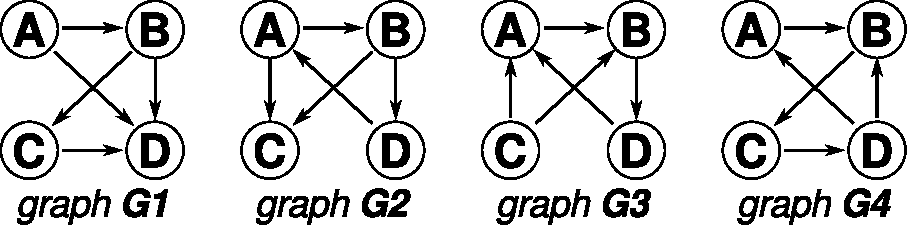
\includegraphics[width=0.6\columnwidth]{q3-graphs.pdf}}\\[1.2\baselineskip]
\noindent
Such graphs can be represented in different ways, for example the two possibilities labeled \textbf{D1} and \textbf{D2} in the boxes below:\\

\noindent
\begin{centering}
\fbox{%
  \begin{minipage}[t]{0.3\columnwidth}
    definition \textbf{D1}\\
    \emph{adjacency lists}\\[1.1\baselineskip]
    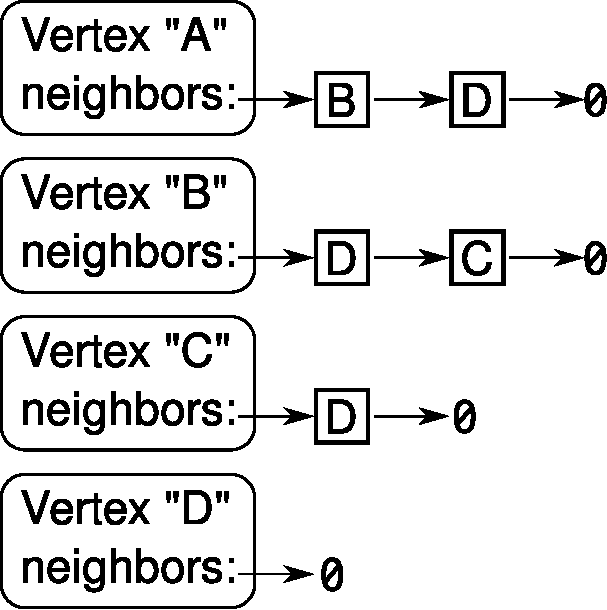
\includegraphics[width=\columnwidth]{q3-adjlist-diagrams.pdf}
  \end{minipage}%
}
\fbox{%
  \begin{minipage}[t]{0.3\columnwidth}
    definition \textbf{D2}\\
    \emph{adjacency matrix}\\[1.1\baselineskip]
    \begin{tabular}{|*{5}{c|}}
      \hline
      \emph{source}
      &
      \multicolumn{4}{l|}{\emph{destination}} \\
        & A & B & C & D \\
      \hline
      A &   & * &   &   \\
      \hline
      B &   &   & * &   \\
      \hline
      C &   &   &   & * \\
      \hline
      D & * & * &   &   \\
      \hline
    \end{tabular}
  \end{minipage}%
}
\end{centering}

\begin{enumerate}
\item
  Which of the graphs \textbf{G1}, \textbf{G2}, \textbf{G3}, or \textbf{G4} is represented by \textbf{D1}?
  And which one is represented by \textbf{D2}?
\item
  For the two graphs that are not represented by either \textbf{D1} or \textbf{D2}, make a sketch of how it would be represented as an adjacency list and as an adjacency matrix.
\item
  Describe the trade-off between adjacency lists and adjacency matrices.
  Under what circumstances is one better than the other?
\end{enumerate}



\section{Graph Representations}

\emph{This group activity is based on question~4 of the written exam from January, 2012.}

The diagram below shows a directed graph.
Its adjacency matrix representation is also given, to define an iteration order for the edges.
This is important because it determines the vertex visitation order for the following questions.
The order is given by reading from left to right along the appropriate row of the adjacency matrix.
\emph{For example, the order of edges emanating from vertex \textbf{C} is: first \textbf{A}, then \textbf{B}, and finally \textbf{F}.}

\begin{center}
  \fbox{%
    \begin{minipage}{0.95\columnwidth}
      \begin{minipage}{0.4\columnwidth}
        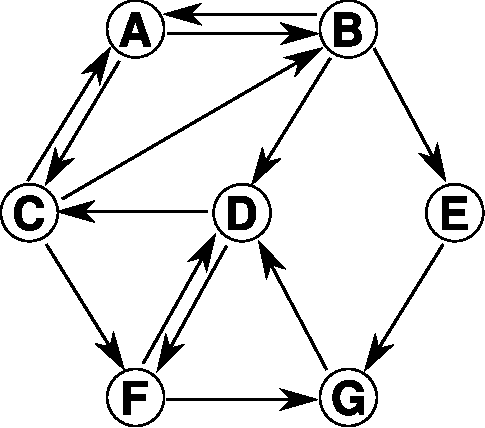
\includegraphics[width=\columnwidth]{q4-graph-diagram.pdf}
      \end{minipage}
      \hfill
      \begin{minipage}{0.45\columnwidth}
        \begin{tabular}{|*{8}{c|}}
          \hline
          \emph{source}
          &
          \multicolumn{7}{l|}{\emph{destination}} \\
            & A & B & C & D & E & F & G \\
          \hline
          A &   & * & * &   &   &   &   \\
          \hline
          B & * &   &   & * & * &   &   \\
          \hline
          C & * & * &   &   &   & * &   \\
          \hline
          D &   &   & * &   &   & * &   \\
          \hline
          E &   &   &   &   &   &   & * \\
          \hline
          F &   &   &   & * &   &   & * \\
          \hline
          G &   &   &   & * &   &   &   \\
          \hline
        \end{tabular}
      \end{minipage}
    \end{minipage}%
  }
\end{center}

\begin{algorithm}
  \caption{
    Breadth-first search: \textbf{BFS}($G,n$)\\
    \textbf{Input:}\\
    -- a directed graph $G$\\
    -- a start vertex $n$
  }\label{algo:bfs}
  \begin{algorithmic}
    \STATE $Q \leftarrow$ empty queue \COMMENT { vertices to be processed }
    \STATE $V \leftarrow$ empty set \COMMENT { visited vertices }
    \STATE enqueue $n$ onto $Q$
    \STATE add $n$ to $V$
    \WHILE { $Q \neq \emptyset$ }
      \STATE $t \leftarrow \text{dequeue}(Q)$
      \STATE process $t$ \COMMENT { e.g.\ print its data }
      \FORALL[visit all outgoing edges] { edges $(t,u)$ }
        \IF[found an unvisited vertex] { $u \notin V$ }
          \STATE add $u$ to $V$
          \STATE enqueue $u$ onto $Q$
        \ENDIF
      \ENDFOR
    \ENDWHILE
  \end{algorithmic}
\end{algorithm}

\begin{algorithm}
  \caption{
    Depth-first search: \textbf{DFS}($G,n$)\\
    \textbf{Input:}\\
    -- a directed graph $G$\\
    -- a start vertex $n$\\
    \textbf{Initializations} before calling DFS():\\
    -- an initially empty set of discovered vertices $D$\\
    -- an initially empty set of explored edges $E$
  }\label{algo:dfs}
  \begin{algorithmic}
    \STATE add $n$ to $D$ \COMMENT { label it ``discovered'' }
    \FORALL[visit all outgoing edges] { edges $e=(n,m)$ }
      \IF[found an unexplored edge] { $e \notin E$ }
        \STATE add $e$ to $E$ \COMMENT { label it ``explored'' }
        \IF[found an undiscovered vertex] { $m \notin D$ }
          \STATE recursively call \textbf{DFS}($G,m$)
        \ENDIF
      \ENDIF
    \ENDFOR
  \end{algorithmic}
\end{algorithm}

\begin{enumerate}
\item
  Perform DFS starting at vertex \textbf{D}.
  Write down the order in which the vertices are visited.
\item
  Perform BFS, also starting at vertex \textbf{D}, and also writing down the visitation order.
\item
  Draw a diagram of the spanning tree rooted at \textbf{A} using depth-first search.
\item
  Draw a diagram of the spanning tree rooted at \textbf{A} using breadth-first search.
\end{enumerate}



\section{Topological Ordering}

\emph{This group activity is based on question~6 of the written exam from October, 2011.}

\paragraph{Definition:}
A \textbf{topological ordering} of a directed graph is a sequence of its vertices such that, for every edge $(u,v)$, $u$ appears before $v$ in the sequence.
Note that for any path from $u$ to $v$, this also implies that $u$ comes before $v$ in the ordering.
In the example graph shown below, the sequence $(C,A,D,B)$ is a topological ordering.

\begin{center}
  \fbox{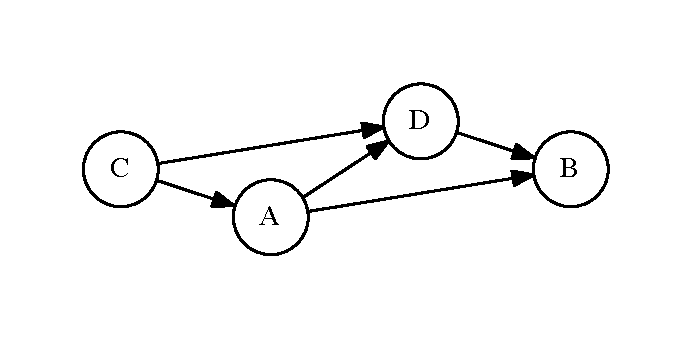
\includegraphics[width=0.3\columnwidth,trim=1cm 1cm 1cm 1cm]{dag-small.pdf}}
\end{center}

\paragraph{Theorem:}
A topological ordering is possible if and only if the graph has no cycles.
In other words, a graph has to be a \textbf{directed acyclic graph} (DAG) in order to have a topological ordering.
And also, every DAG has at least one topological ordering.

\begin{enumerate}
\item
  The class is subdivided into two groups.
  Discuss how you can prove the theorem.
\item
  Each student individually should apply Kahn's Algorithm (shown in Listing~\ref{algo:kahn}) to the two graphs in Figure~\ref{fig:graphs}.
  Then compare your results with someone else in your group.
\end{enumerate}

\begin{algorithm}
  \caption{
    Kahn's Algorithm\\
    \textbf{Input:} a directed graph $G$
  }\label{algo:kahn}
  \begin{algorithmic}
    \STATE $L \leftarrow$ empty list \COMMENT { will contain the topological order }
    \STATE $S \leftarrow$ set of nodes that have \textbf{no incoming} edges
    \WHILE { $S \neq \emptyset$ }
      \STATE remove a node $n$ from $S$
      \STATE insert $n$ into $L$
      \FORALL [visit all outgoing edges] { edges $e = (n,m)$ }
        \STATE remove $e$ from $G$
        \IF { $m$ has no more incoming edges }
          \STATE insert $m$ into $S$
        \ENDIF
      \ENDFOR
    \ENDWHILE
    \IF { $G$ has edges }
      \RETURN error \COMMENT { $G$ has at least one cycle }
    \ENDIF
    \RETURN $L$
  \end{algorithmic}
\end{algorithm}

\begin{figure}
  \centering
  \fbox{
    \begin{minipage}{0.35\columnwidth}
      \centering
      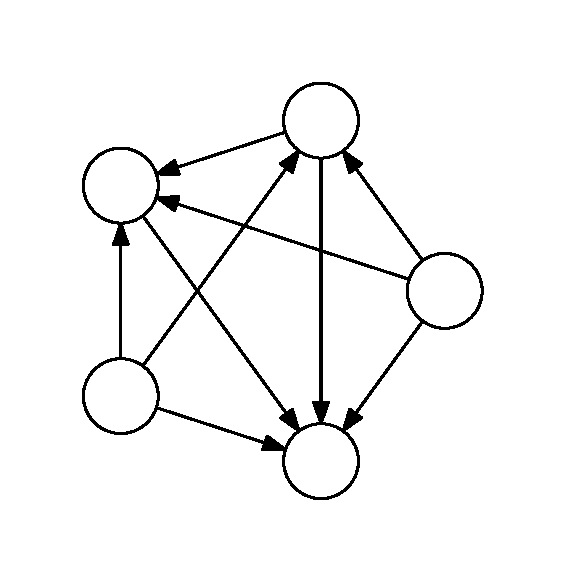
\includegraphics[width=\columnwidth,trim=1cm 1cm 1cm 1cm]{cycle-detection-dag.pdf}
      \textbf{graph A}
    \end{minipage}}
  \fbox{
    \begin{minipage}{0.35\columnwidth}
      \centering
      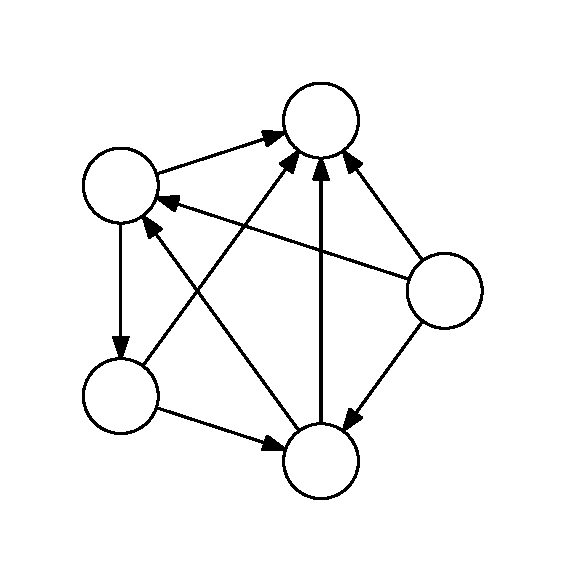
\includegraphics[width=\columnwidth,trim=1cm 1cm 1cm 1cm]{cycle-detection-non-dag.pdf}
      \textbf{graph B}
    \end{minipage}}
  \caption{Example graphs for topological ordering}\label{fig:graphs}
\end{figure}


\end{document}
